\documentclass[5pt]{article}
\usepackage{mathptmx,amsmath}
\usepackage{pdfslide2,pause}
\usepackage{eurosym}
\usepackage[portuguese,english]{babel}
%\usepackage{kerkis}
\usepackage{colortbl} % used to highlight row or columns of tables. http://www.tug.org/pracjourn/2007-1/mori/mori.pdf
\usepackage[small]{caption} % more option on http://www.dd.chalmers.se/latex/Docs/PDF/caption.pdf
\usepackage[tight,scriptsize]{subfigure}
\usepackage{lastpage}
\usepackage{chngcntr}
\usepackage[absolute,overlay]{textpos}
\usepackage{tabto}
\usepackage{animate}
\usepackage{multirow}
%\usepackage{listings}
\captionsetup{labelformat=empty,skip=-0.8cm}

%%%% Diamantino %%%%
% As minhas packages
\usepackage[utf8]{inputenc}
\usepackage{braket}

%\lstset{
%    language=Matlab,                % choose the language of the code
%    basicstyle=\ttfamily\tiny,      % the size of the fonts that are used for the code
%    numbers=none,                   % where to put the line-numbers
%    numberstyle=\tiny,              % the size of the fonts that are used for the line-numbers
%    stepnumber=1,                   % the step between two line-numbers. If it's 1 each line will be numbered
%    numbersep=5pt,                  % how far the line-numbers are from the code
%    backgroundcolor=\color{white},  % choose the background color. You must add \usepackage{color}
%    showspaces=false,               % show spaces adding particular underscores
%    showstringspaces=false,         % underline spaces within strings
%    showtabs=false,                 % show tabs within strings adding particular underscores
%    tab=\rightarrowfill,
%    frame=none,	                 % adds a frame around the code
%    tabsize=2,	                     % sets default tabsize to 2 spaces
%    captionpos=b,                   % sets the caption-position to bottom
%    breaklines=true,                % sets automatic line breaking
%    breakatwhitespace=false,        % sets if automatic breaks should only happen at whitespace
%    title=\lstname,                 % show the filename of files included with \lstinputlisting; also try caption instead of title
%    escapeinside={\%*}{*)},          % if you want to add a comment within your code
%    morekeywords={ifftshift,fftshift},
%    keywordstyle=\bfseries\color[rgb]{0,0,0.3},
%    commentstyle=\color[rgb]{0.133,0.5,0.133}
%}
%\lstset{
%    emph={function,end,for,if,while},
%    emphstyle=\bfseries\color[rgb]{0.6,0,0},
%}

\definecolor{itblue}{rgb}{0.0,0.0,0.5}
\definecolor{itred}{rgb}{0.82,0.18,0.24}
\newcommand{\pageNum}{
    \begin{picture}(0,0)(0,0)
        \put(-15,-390){
            \begin{minipage}{1.8cm}
            \end{minipage}
        }
    \end{picture}
}
\newcommand{\cb}[1]{{\color{itblue} #1}}%
\newcommand{\cred}[1]{{\color{itred} #1}}%
\newcommand{\bb}[1]{{\textbf{\color{itblue} #1}}}%
\newcommand{\br}[1]{{\textbf{\color{itred} #1}}}%
\renewcommand{\labelitemi}{\textcolor{itred}{\normalsize $\bullet$}}
\renewcommand{\labelitemii}{\textcolor{itblue}{$\bullet$}}
\newcommand{\mysection}[1]{\section*{\pageNum\color{itred}\sffamily #1}\vspace*{0.5cm}\overlay{./figures/it_1.png}\sffamily}%
\newcommand{\ITfootnote}[1]{\hspace{1.8cm}\begin{minipage}{13cm}\tiny{#1}\end{minipage}}
\newcommand{\edfaGain}{$G=\exp\left(\frac{\alpha}{2}L_{span}\right)$}
\newenvironment{reference}{
    \begin{textblock*}{0.7\textwidth}(32mm,137mm)\tiny\noindent\bgroup\color{black}
}
{
    \egroup\end{textblock*}
}


\graphicspath{{./figures/}}
\pagestyle{title}

\hyphenpenalty=50000
\tolerance=10000

\setlength{\textheight}{1.5\textheight}

%%%%%%%%%%%%%%%%%%%%%%%%%%%%%%%%%%%%%%%%%%%%%%%%%%%%%%%%%%%%%%%%%%%%%%%%%%%%%%%%%%%%%%%%%%%%%%%%%%%
%%%%%%%%%%%%%%%%%%%%%%%%%%%%%%%%%%%%%%%%%%%%%%%%%%%%%%%%%%%%%%%%%%%%%%%%%%%%%%%%%%%%%%%%%%%%%%%%%%%

\begin{document}

%************************************************************************************************
%                                          SLIDE
%************************************************************************************************
\pagenumbering{roman}
\begin{titlepage}  \overlay{./figures/it_0.png}

\color{itblue} \sffamily \noindent \small
\hspace*{1cm}  Universidade de Aveiro\\ %Instituto\\ Superior T�cnico, Instituto de Telecomunica��es\\
\hspace*{1cm}  2017-2018\\ %Lisboa, 14th of February, 2013\\

\vspace*{1cm}
\begin{center}
    \color{black} \sffamily \noindent \Large
    \br{CV-QKD System\\}
\end{center}
\vspace{6mm}
\begin{center}
    \color{black}
    \textbf{Daniel Pereira\\}
    {(danielfpereira@ua.pt)}
\end{center}

\vspace{0.0mm}
\scriptsize
\begin{center}
Department of Electronics, Telecommunications and Informatics,\\
University of Aveiro, Aveiro, Portugal\\
Instituto de Telecomunicações, Aveiro, Portugal\\
\end{center}

\vspace{1.0cm}
\hfill \tiny \copyright 2017, it - instituto de telecomunicações\hfill

\end{titlepage}


\renewcommand{\headsep}{-25pt}
\pagenumbering{arabic}



%--------------------------------------------------------------------------------------------------
%------------ SLIDE-------
\mysection{Introduction - Objectives}\large
\vspace{0cm}

\begin{itemize}
\item Study pilot-aided, locally generated Local Oscillator Continuous Variables Quantum Key Distribution (CV-QKD) with 4 state discrete modulation.
\item Both simulation and experimental results where obtained.
\item Results where linked to theoretical expected values, not each other (missing detector information to compare simulation to experimental values).
\end{itemize}

%--------------------------------------------------------------------------------------------------
%------------ SLIDE-------
%\mysection{Introduction - Content in this presentation}\large
%\vspace{0cm}
%
%\begin{itemize}
%\item Simulation results:
%\begin{itemize}
%\item Noise characterization.
%\item Secret key generation rate in function of transmission for two levels of excess noise.
%\end{itemize}
%\item Experimental results:
%\begin{itemize}
%\item Phase drift compensation.
%\item Noise characterization experiment.
%\item Key distribution experiment with secret key generation rate estimation.
%\end{itemize}
%\end{itemize}


%--------------------------------------------------------------------------------------------------
%------------ SLIDE-------
\mysection{Theoretical notes - Security of CV-QKD}\large
\vspace{0cm}

\noindent
In CV-QKD, the key for a One Time Pad (OTP) protocol is shared through a quantum channel. The security of this key is evaluated in terms of secret key generation rate (bits/symbol):
\begin{equation}
K=\beta I(A:B)-S(B:E).
\end{equation}
The rate is positive if Alice and Bob manage to share more information, $I(A:B)$, than the information obtained by Eve on Bob's results, $S(B:E)$. $\beta$ represents the efficiency of the employed error correction.


%--------------------------------------------------------------------------------------------------
%------------ SLIDE-------
%\mysection{Theoretical notes - Estimating information rates}\large
%\vspace{0cm}
%
%\noindent
%The mutual classical information is estimated as:
%\begin{equation}
%I(A:B)=\log_2\left(1+\frac{T\braket{n}}{1+\frac{T}{2}\epsilon}\right).
%\end{equation}
%This definition of $I(A:B)$ assumes a Gaussian modulated signal, while we use discrete modulation. The effect of this inaccuracy on the mutual information is included in the error correction efficiency $\beta$.\\

%--------------------------------------------------------------------------------------------------
%------------ SLIDE-------
\mysection{Theoretical notes - Estimating information rates}\large
\vspace{0cm}

\noindent
The quantum information Eve possesses, $S(B:E)$, is upper bounded by the quantum information between Alice and Bob, $S(B:A)$, which can be estimated by knowledge of the covariance matrices.
\begin{equation}
\gamma_\text{AB}=\left[
\begin{matrix}
(1+2\braket{n})\mathbb{I}_2 & \sqrt{\frac{T}{2}}Z\sigma_Z \\
\sqrt{\frac{T}{2}}Z\sigma_Z & \left(T\braket{n}+1+\frac{T}{2}\varepsilon\right)\mathbb{I}_2 \\
\end{matrix}
\right]
\end{equation}
\begin{equation}
\gamma_{AB|B}=\left((1+2\braket{n})-\frac{\frac{T}{2}Z^2}{T\braket{n}+2+\frac{T}{2}\epsilon}\right)\mathbb{I}_2
\end{equation}
The quantum information can then be calculated from the symplectic eigenvalues of the two previous covariance matrices.

%--------------------------------------------------------------------------------------------------
%------------ SLIDE-------
%\mysection{Theoretical notes - Estimating information rates}\large
%\vspace{0cm}
%
%\noindent
%The quantum information can then be calculated from the symplectic eigenvalues of the two previous covariance matrices through:
%\begin{equation}
%\begin{aligned}
%S(B:E)=&\sum_{k=1}^2\left[(\bar{n}_k^{AB}+1)\log_2(\bar{n}_k^{AB}+1)-\bar{n}_k^{AB}\log_2\bar{n}_k^{AB}\right]\\
%&-(\bar{n}^{AB|B}+1)\log_2(\bar{n}^{AB|B}+1)-\bar{n}^{AB|B}\log_2\bar{n}^{AB|B},
%\end{aligned}
%\end{equation}
%where $\bar{n}=(\mu-1)/2$, with $\mu$ representing the symplectic eigenvalues.


%--------------------------------------------------------------------------------------------------
%------------ SLIDE-------
\mysection{Theoretical notes - Security of practical CV-QKD}\large
\vspace{0cm}

\noindent
Taking into account the need to estimate the channel parameters, the covariance matrices are altered to:
\begin{equation}
\gamma_\varepsilon=\left[
\begin{matrix}
(1+2\braket{n})\mathbb{I}_2 & t_\text{min}Z\sigma_z \\
t_\text{min}Z\sigma_z & \left(2t_\text{min}^2\braket{n}+\sigma_\text{max}^2\right)\mathbb{I}_2
\end{matrix}
\right],
\end{equation}
\begin{equation}
\gamma_{AB|B_\varepsilon}=\left(1+2\braket{n}-\frac{t_\text{min}^2Z^2}{2t_\text{min}^2\braket{n}+1+\sigma_\text{max}^2}\right)\mathbb{I}_2.
\end{equation}
$t_\text{min}$ is the minimum value of $t=\sqrt{\frac{T}{2}}$ except with a probability of $\Delta/2$.\\
$\sigma_\text{max}^2$ is the maximum value of $\sigma^2=1+\frac{T}{2}\epsilon$ except with a probability of $\Delta/2$.\\
~\\
This is dubbed the \textbf{finite size analysis}.\\

%--------------------------------------------------------------------------------------------------
%------------ SLIDE-------
\mysection{Simulation - Block diagram}\large
\vspace{0cm}

\begin{center}
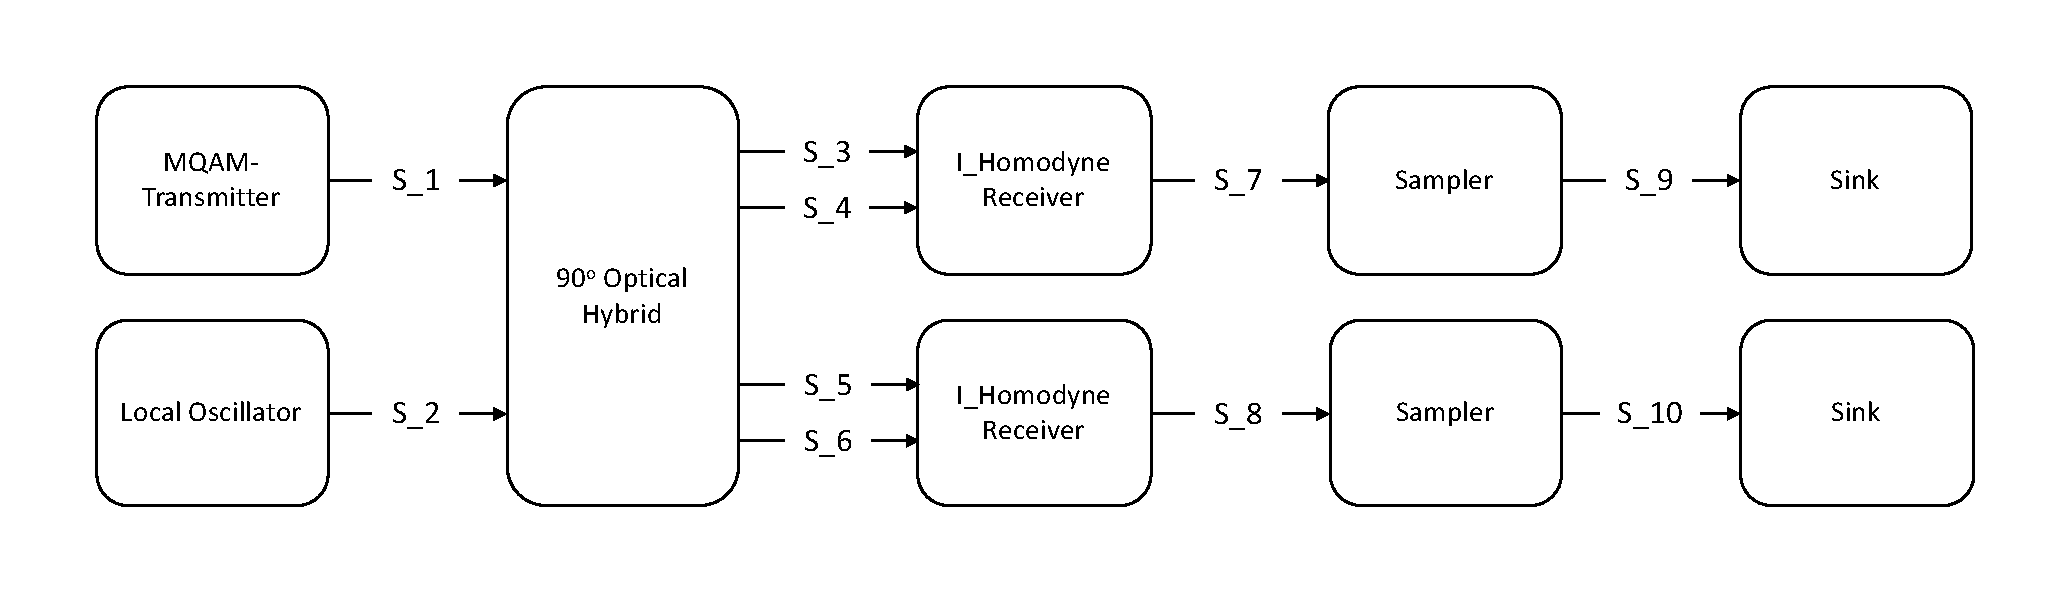
\includegraphics[width=\linewidth, trim={1cm 1cm 1cm 1cm}, clip=true]{diagramSIMU.pdf}
\end{center}
\begin{minipage}{.5\textwidth}
  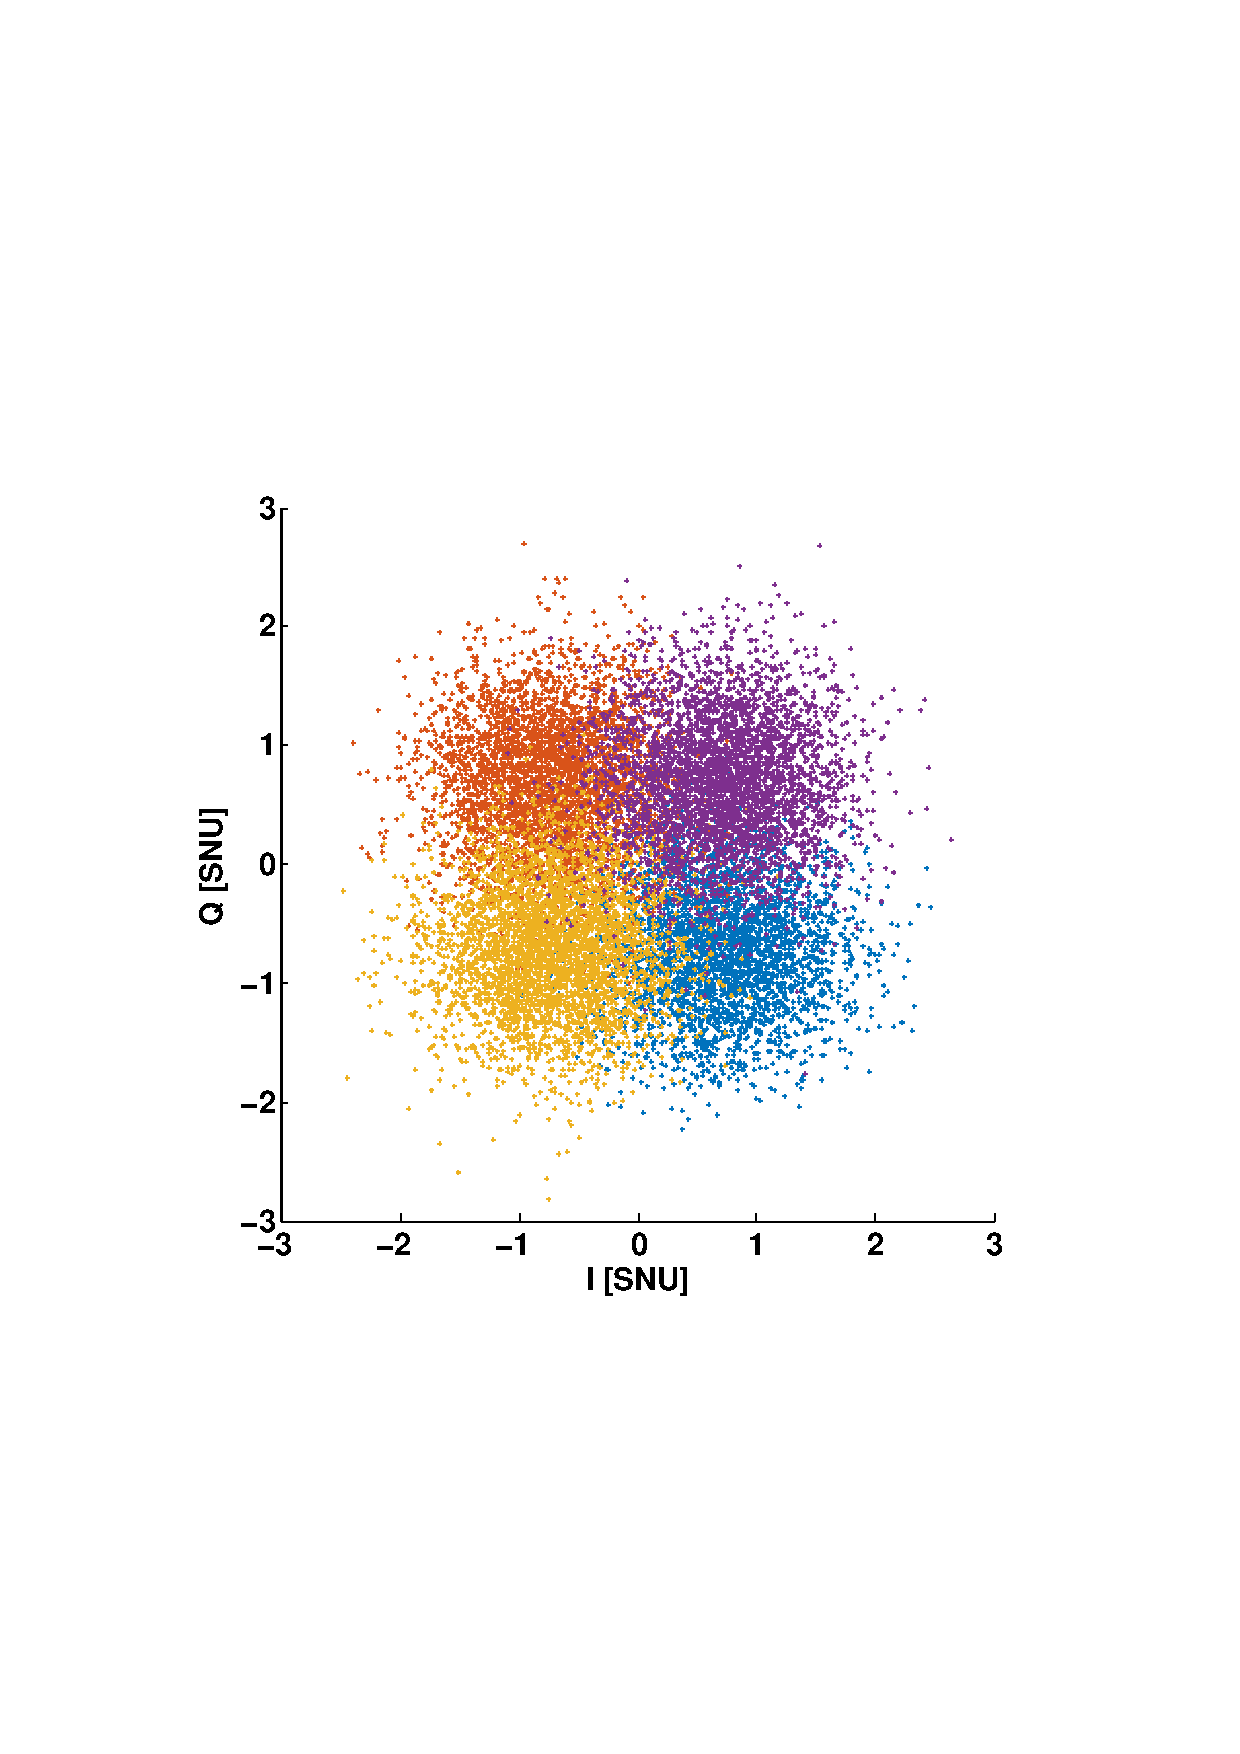
\includegraphics[width=\linewidth, trim={1cm 7cm 1.5cm 8cm}, clip=true]{constellationSimulation.pdf}
\end{minipage}% This must go next to `\end{minipage}`
\begin{minipage}{.5\textwidth}
  \noindent
  Two independent noise sources are considered:
  \begin{itemize}
  	\item Thermal noise.
  	\item Shot noise. 
  \end{itemize}   
\end{minipage}

%--------------------------------------------------------------------------------------------------
%------------ SLIDE-------
\mysection{Simulation - Detector noise characterization}\large
\vspace{0cm}

\noindent
The first results presented here pertain to a noise variance characterization of the simulated homodyne receiver:\\
\begin{minipage}{.5\textwidth}
  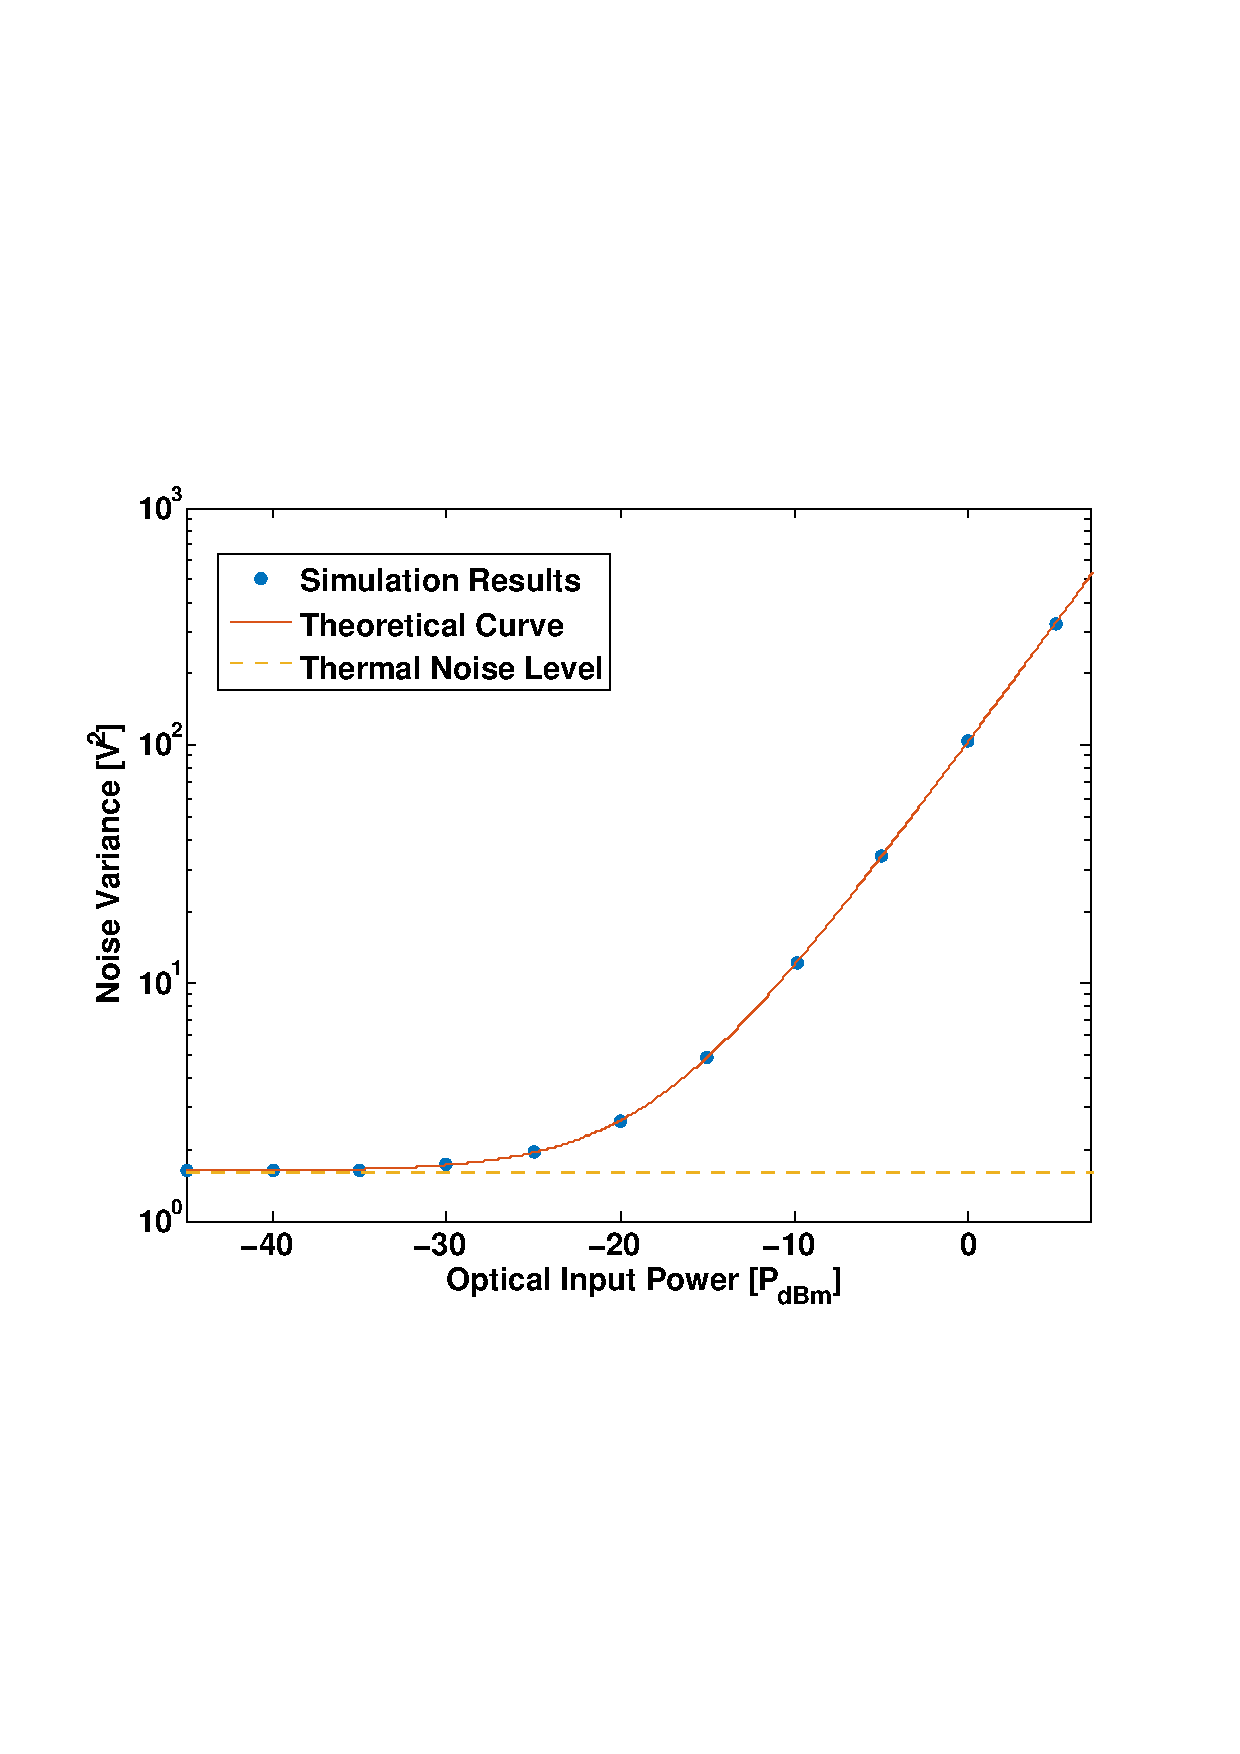
\includegraphics[width=\linewidth, trim={1cm 7cm 1.5cm 8cm}, clip=true]{simucharact.pdf}
\end{minipage}% This must go next to `\end{minipage}`
\begin{minipage}{.5\textwidth}
  \noindent
  The simulation results closely follow the theoretical expectation values for all the studied power levels. 
  The linear dominated stage of the detector is seen to start at a Local Oscillator optical input power of -15 dBm.
\end{minipage}

%--------------------------------------------------------------------------------------------------
%------------ SLIDE-------
\mysection{Simulation - Secret key generation rate}\large
\vspace{0cm}

\noindent
Following the noise characterization, the secret key generation rate of the simulation was evaluated and compared to the theoretical expectation values:\\
\begin{minipage}{.5\textwidth}
  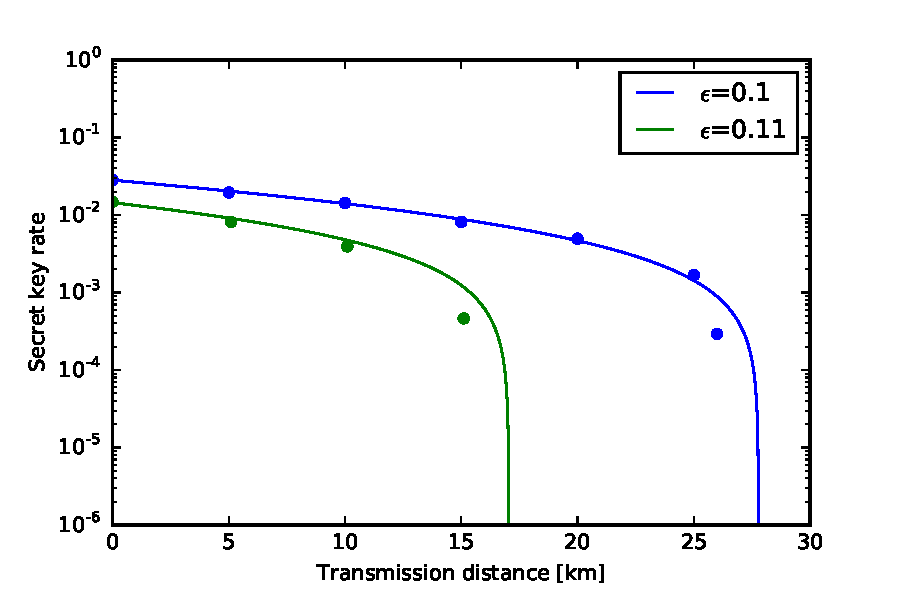
\includegraphics[width=\linewidth, clip=true]{keyratesimulation.pdf}
\end{minipage}% This must go next to `\end{minipage}`
\begin{minipage}{.5\textwidth}
  \noindent
  The simulation results closely follow the theoretical curve just until when the curve starts to quickly tend to 0, at which point they diverge.
\end{minipage}
Theoretical (full line) and simulation (dots) results for secret key generation, reconciliation efficiency set at $\beta$=80\% and transmission given by $T=10^{-0.02d}$ ($d$ is the transmission distance in kilometres).
%Theoretical (full line) and simulation (dots) results for secret key generation, reconciliation efficiency set at $\beta$=80\% and transmission given by $T=10^{−0.02d}$ ($d$ is the transmission distance in kilometres).

%--------------------------------------------------------------------------------------------------
%------------ SLIDE-------
\mysection{Experimental results - Experimental system}\large
\vspace{0cm}

\begin{center}
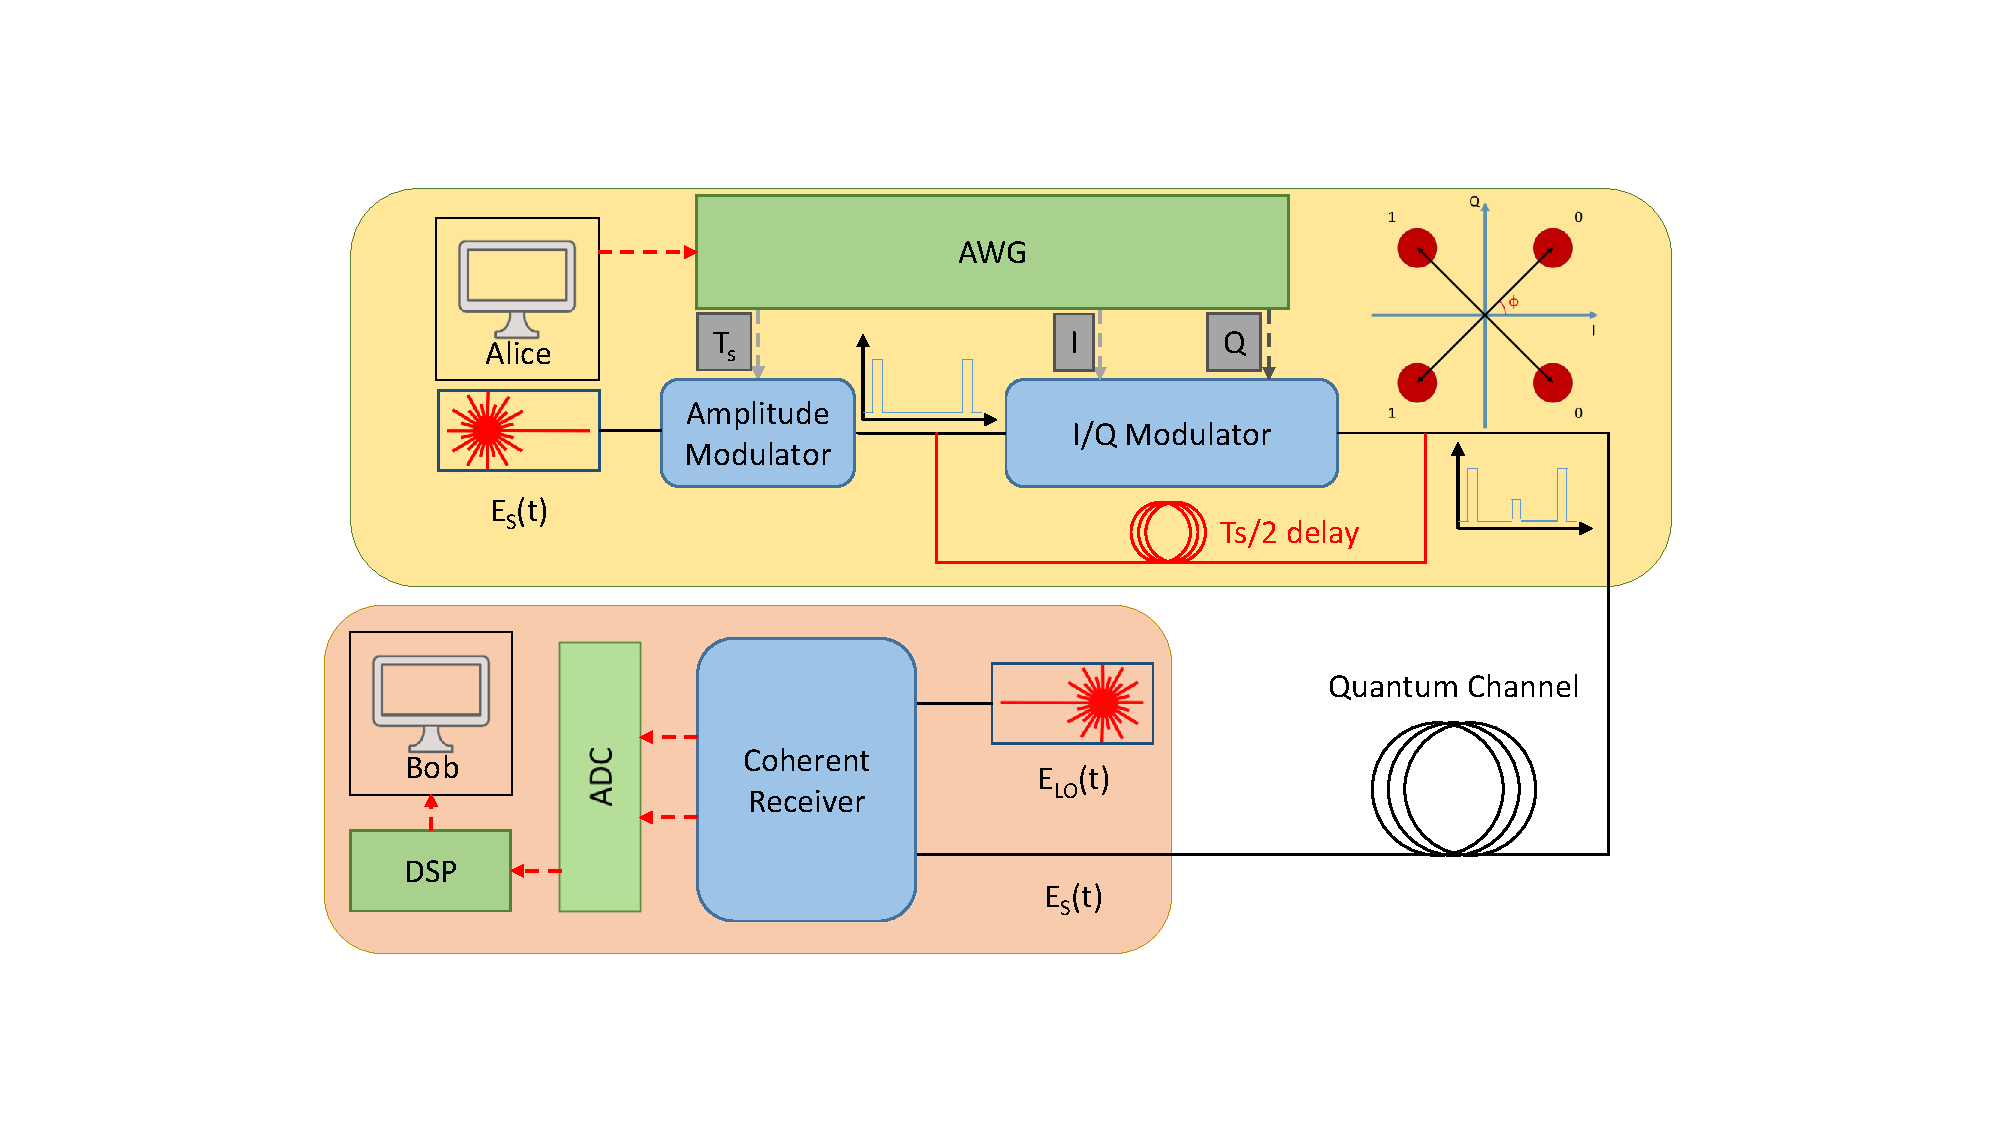
\includegraphics[width=\linewidth, trim={1cm 1cm 1cm 1cm}, clip=true]{withtrace.pdf}
\end{center}


%--------------------------------------------------------------------------------------------------
%------------ SLIDE-------
\mysection{Experimental results - Output data processing}\large
\vspace{0cm}

\noindent
The following digital signal processing was employed:\\
\begin{minipage}{.5\textwidth}
  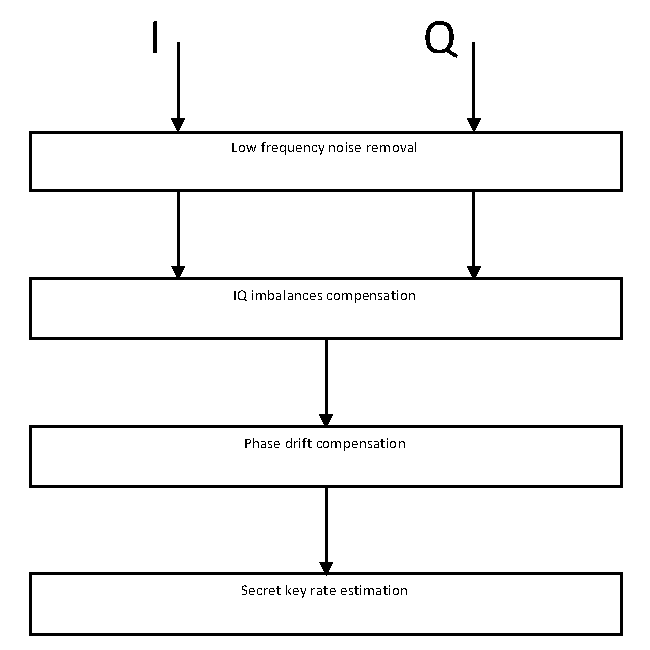
\includegraphics[width=\linewidth]{farukstylediagram.pdf}
\end{minipage}% This must go next to `\end{minipage}`
\begin{minipage}{.5\textwidth}
  \noindent
  \begin{itemize}
  \item The IQ imbalances are removed by applying a Gram-Schmidt orthogonalization process.
  \item The phase drift is compensated by measuring the relative phase between the two lasers and removing that value from the decoded results.
  \item The secret key rate is estimated through the finite size analysis method presented above.
  \end{itemize}
\end{minipage}


%--------------------------------------------------------------------------------------------------
%------------ SLIDE-------
\mysection{Experimental results - Phase drift compensation}\large
\vspace{0cm}

\begin{minipage}{.5\textwidth}
  \noindent
  The phase drift compensation scheme was tested.\\
  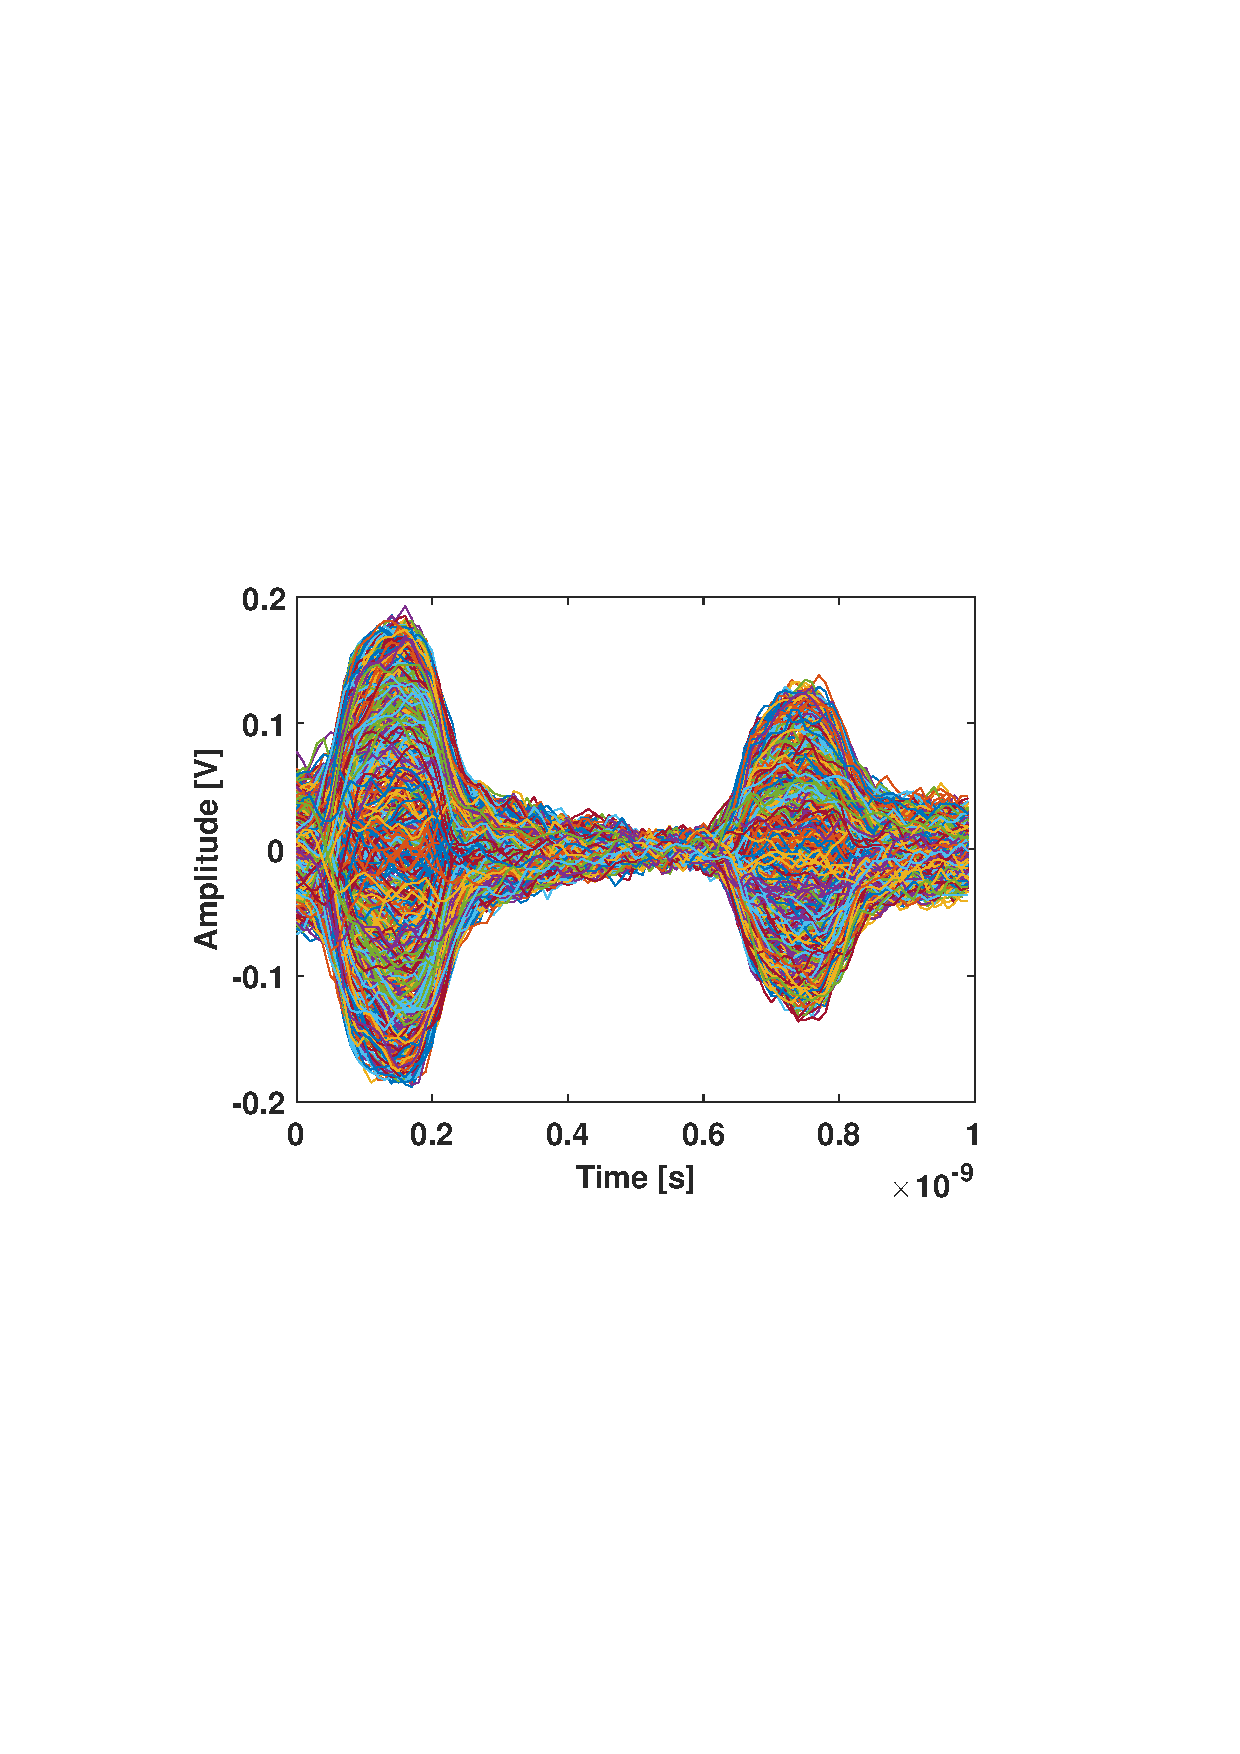
\includegraphics[width=\linewidth, trim={3cm 9cm 3cm 9.5cm}, clip=true]{persistence2.pdf}
\end{minipage}% This must go next to `\end{minipage}`
\begin{minipage}{.5\textwidth}
\begin{center}
  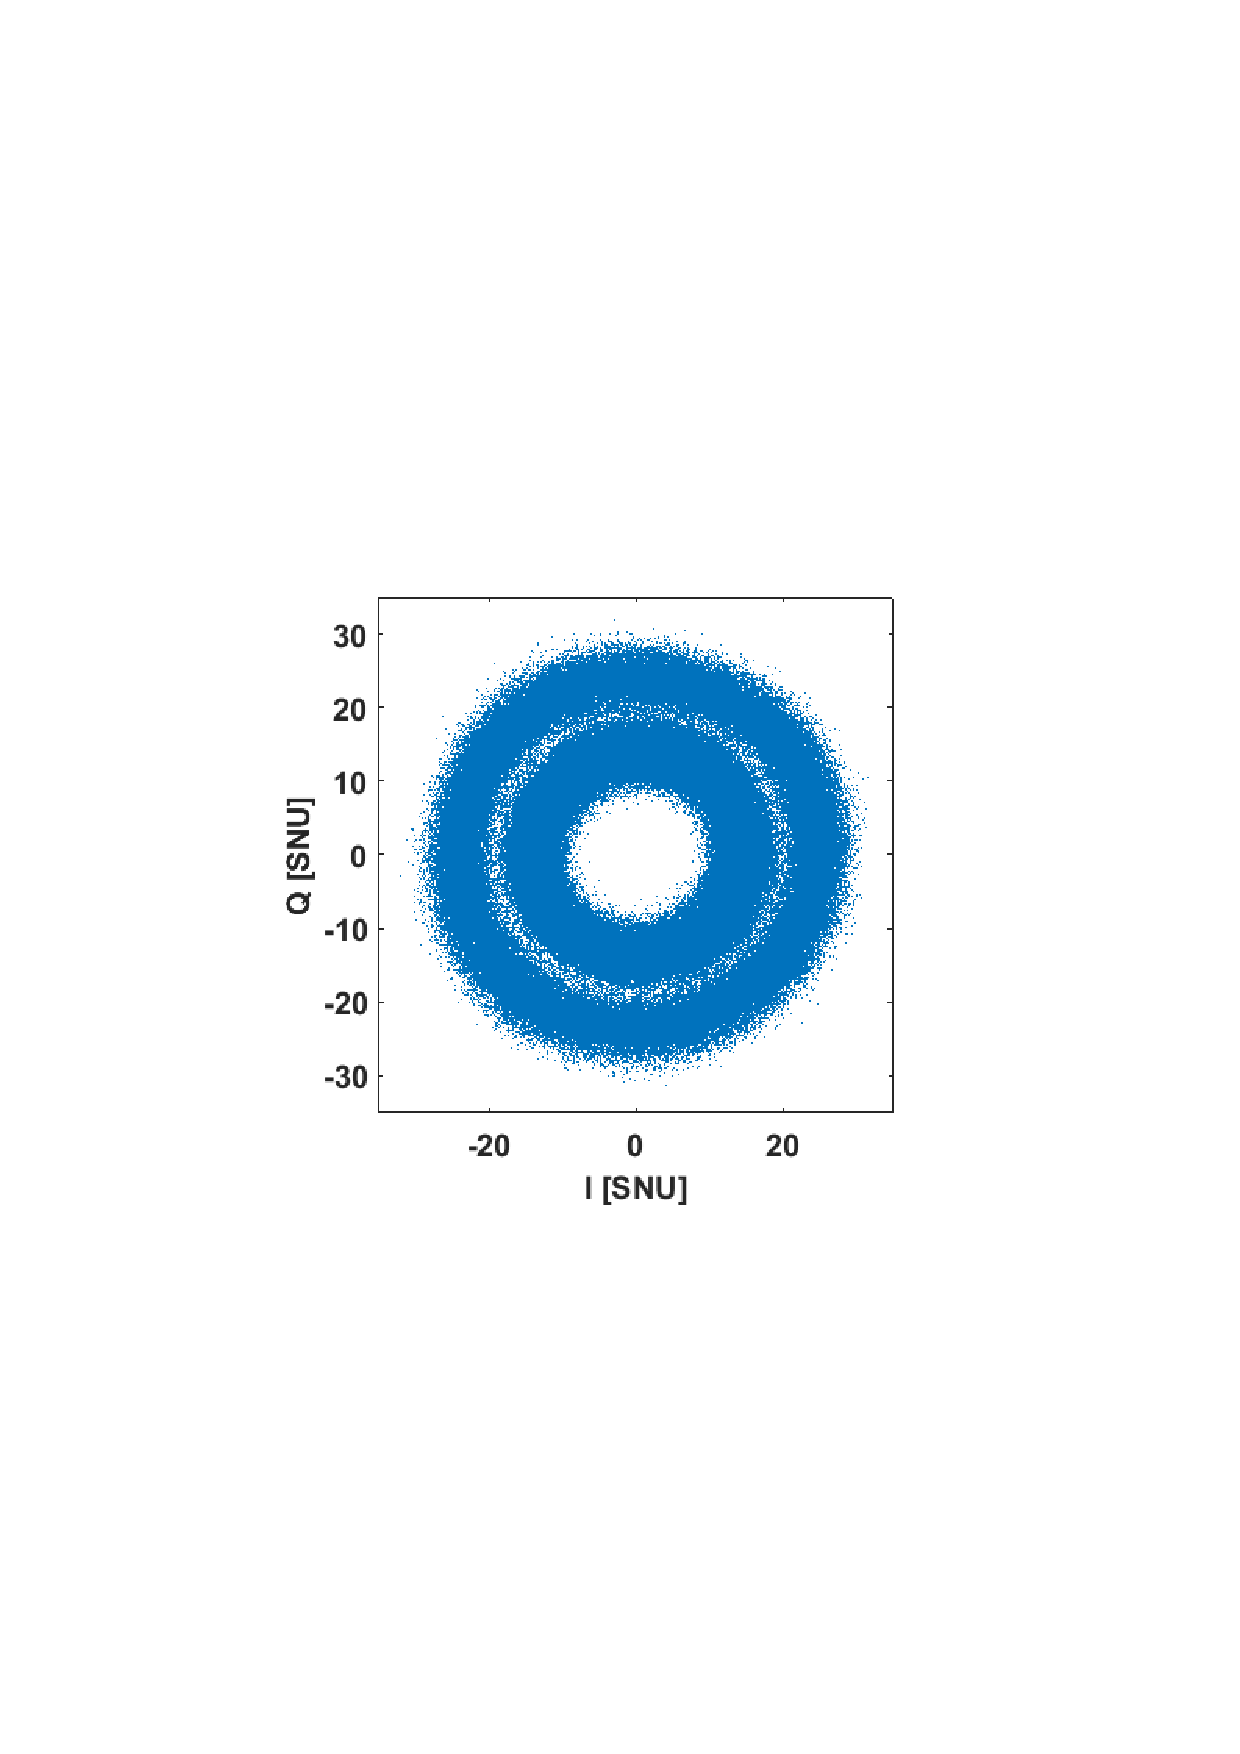
\includegraphics[width=.73\linewidth, trim={3cm 9cm 3cm 9.5cm}, clip=true]{doubleBTBSNUBefPhasDriftComp.pdf}\\
  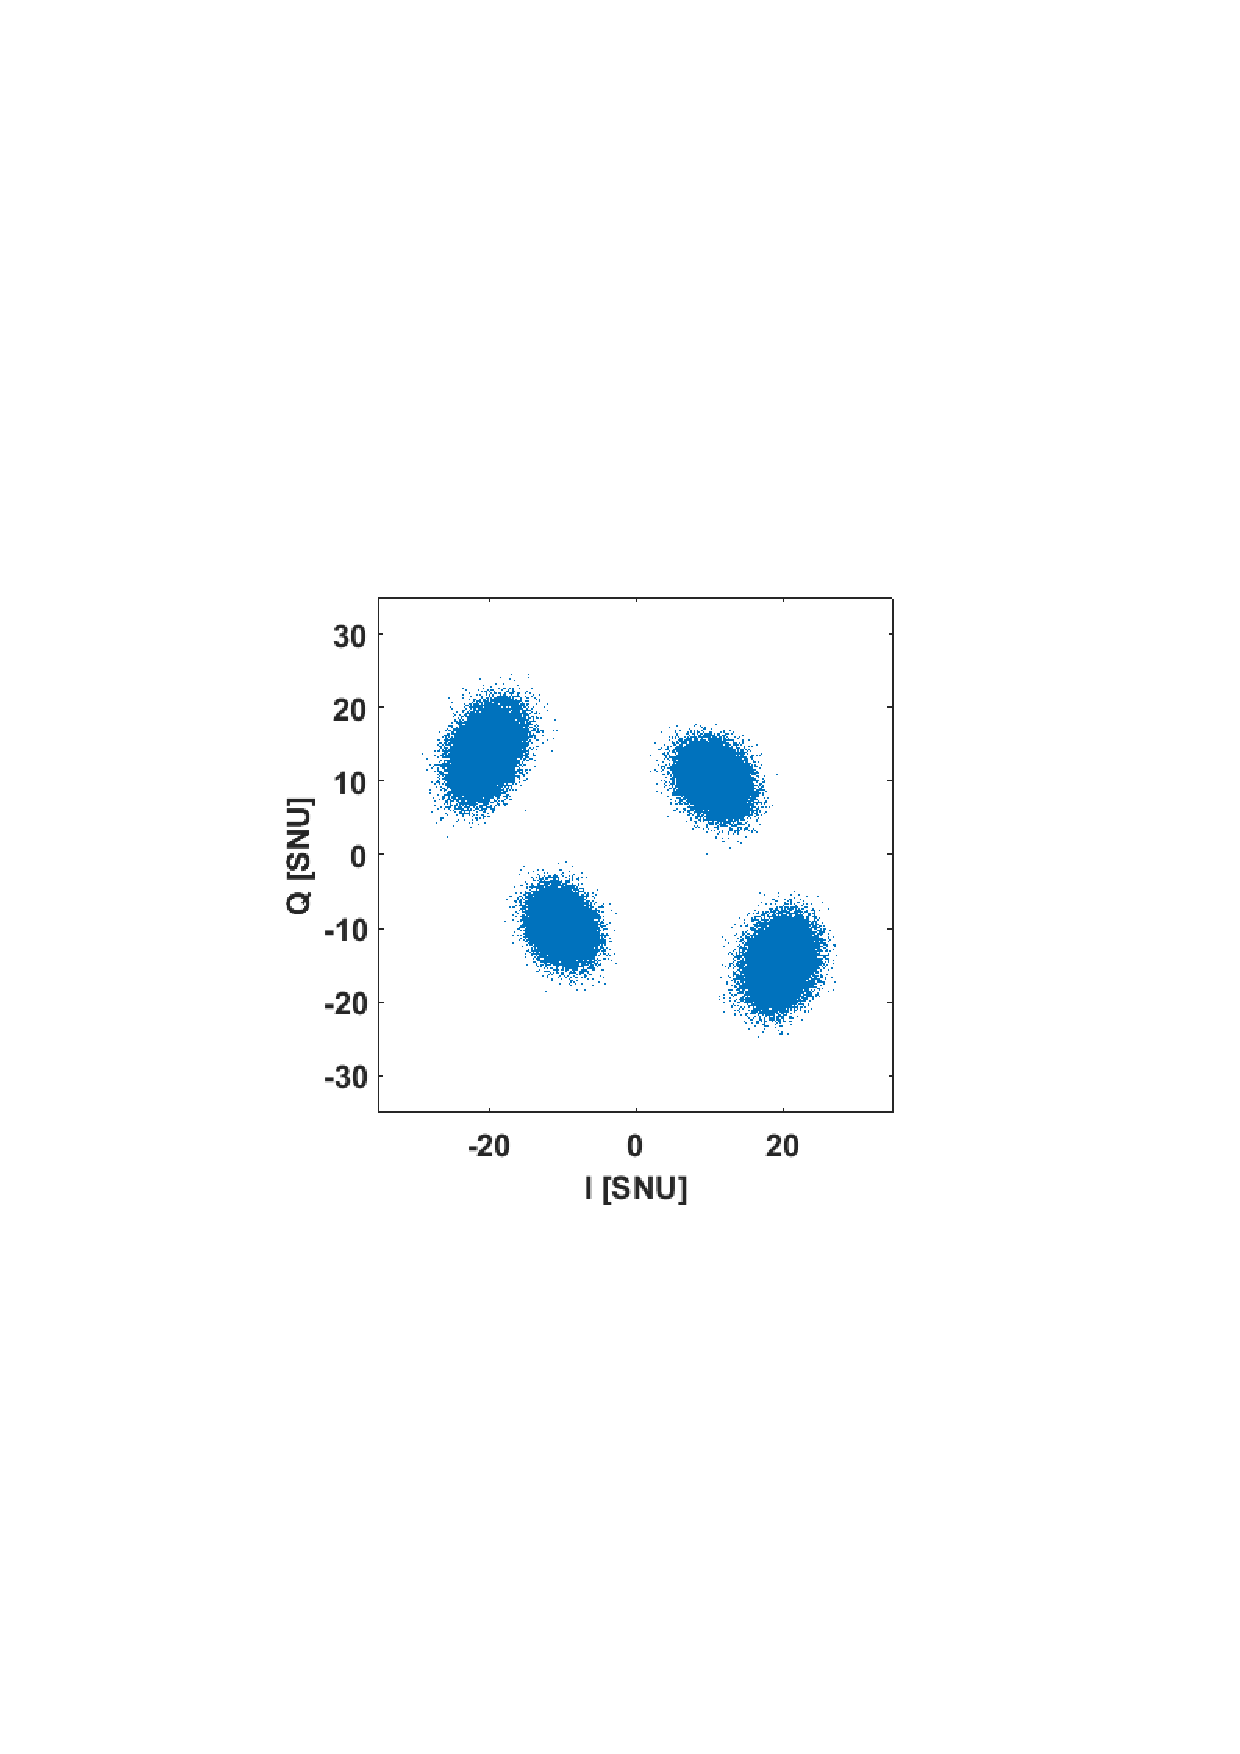
\includegraphics[width=.73\linewidth, trim={3cm 9cm 3cm 9.5cm}, clip=true]{doubleBTBSNU.pdf}
\end{center}
\end{minipage}

%--------------------------------------------------------------------------------------------------
%------------ SLIDE-------
\mysection{Experimental results - Detector noise characterization}\large
\vspace{0cm}

\noindent
A shot noise characterization of the detector was performed

\begin{minipage}{.5\textwidth}
 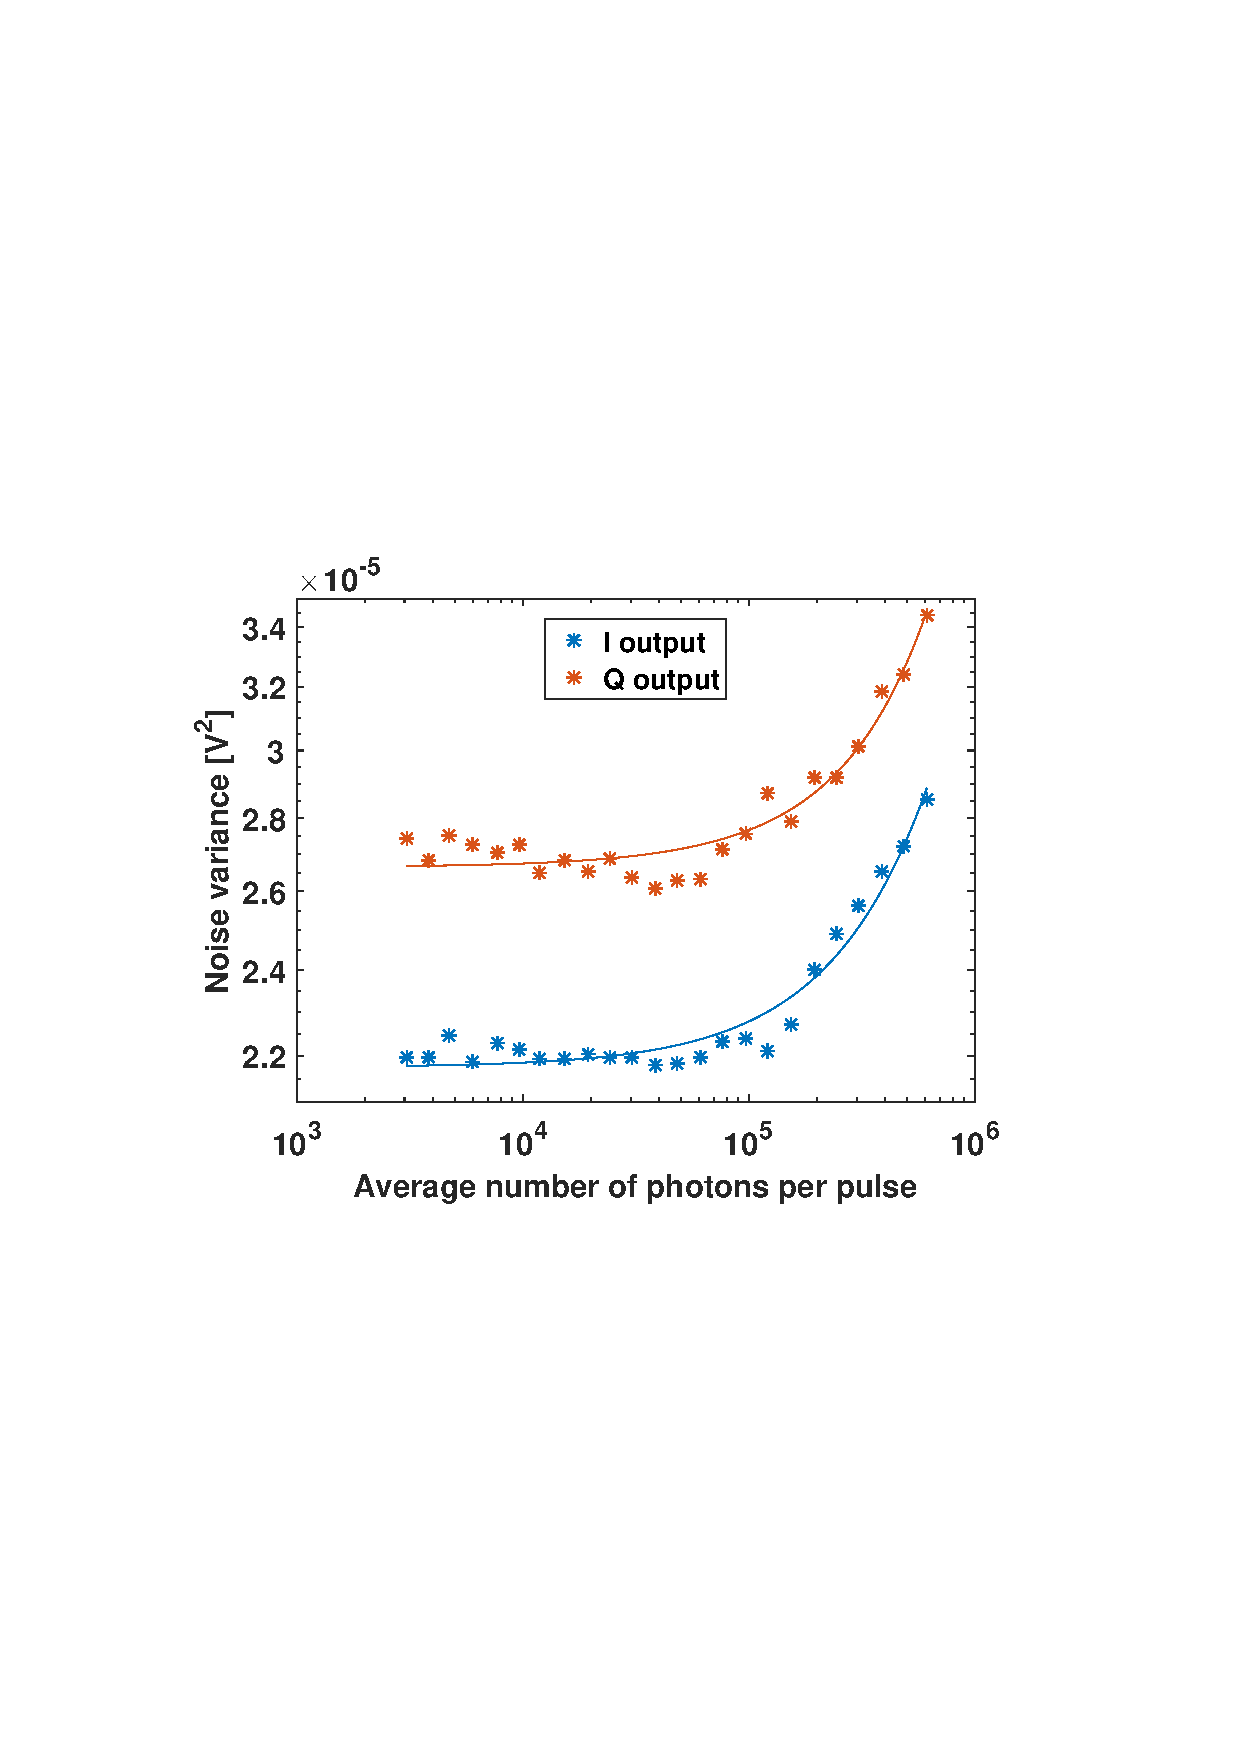
\includegraphics[width=\linewidth, trim={3cm 9cm 3cm 9cm}, clip=true]{characterizationInputLO.pdf}
\end{minipage}% This must go next to `\end{minipage}`
\begin{minipage}{.5\textwidth}
\begin{itemize}
\item The linear was stage was found to be below $\braket{n}\sim4\times10^6$.
\item Our detector has a very short linear stage, not ideal for this application.
\item Shot Noise Units (SNU) conversion factor was obtained.
\end{itemize}
\end{minipage}


%--------------------------------------------------------------------------------------------------
%------------ SLIDE-------
\mysection{Experimental results - System performance}\large
\vspace{0cm}

\noindent
The system's performance was evaluated for 4 different setups, utilizing a single/double laser setup coupled with either a direct connection or a 10~km transmission channel. The secret key rate was estimated through the finite size analysis presented before.

\begin{minipage}{.5\textwidth}
\begin{center}
 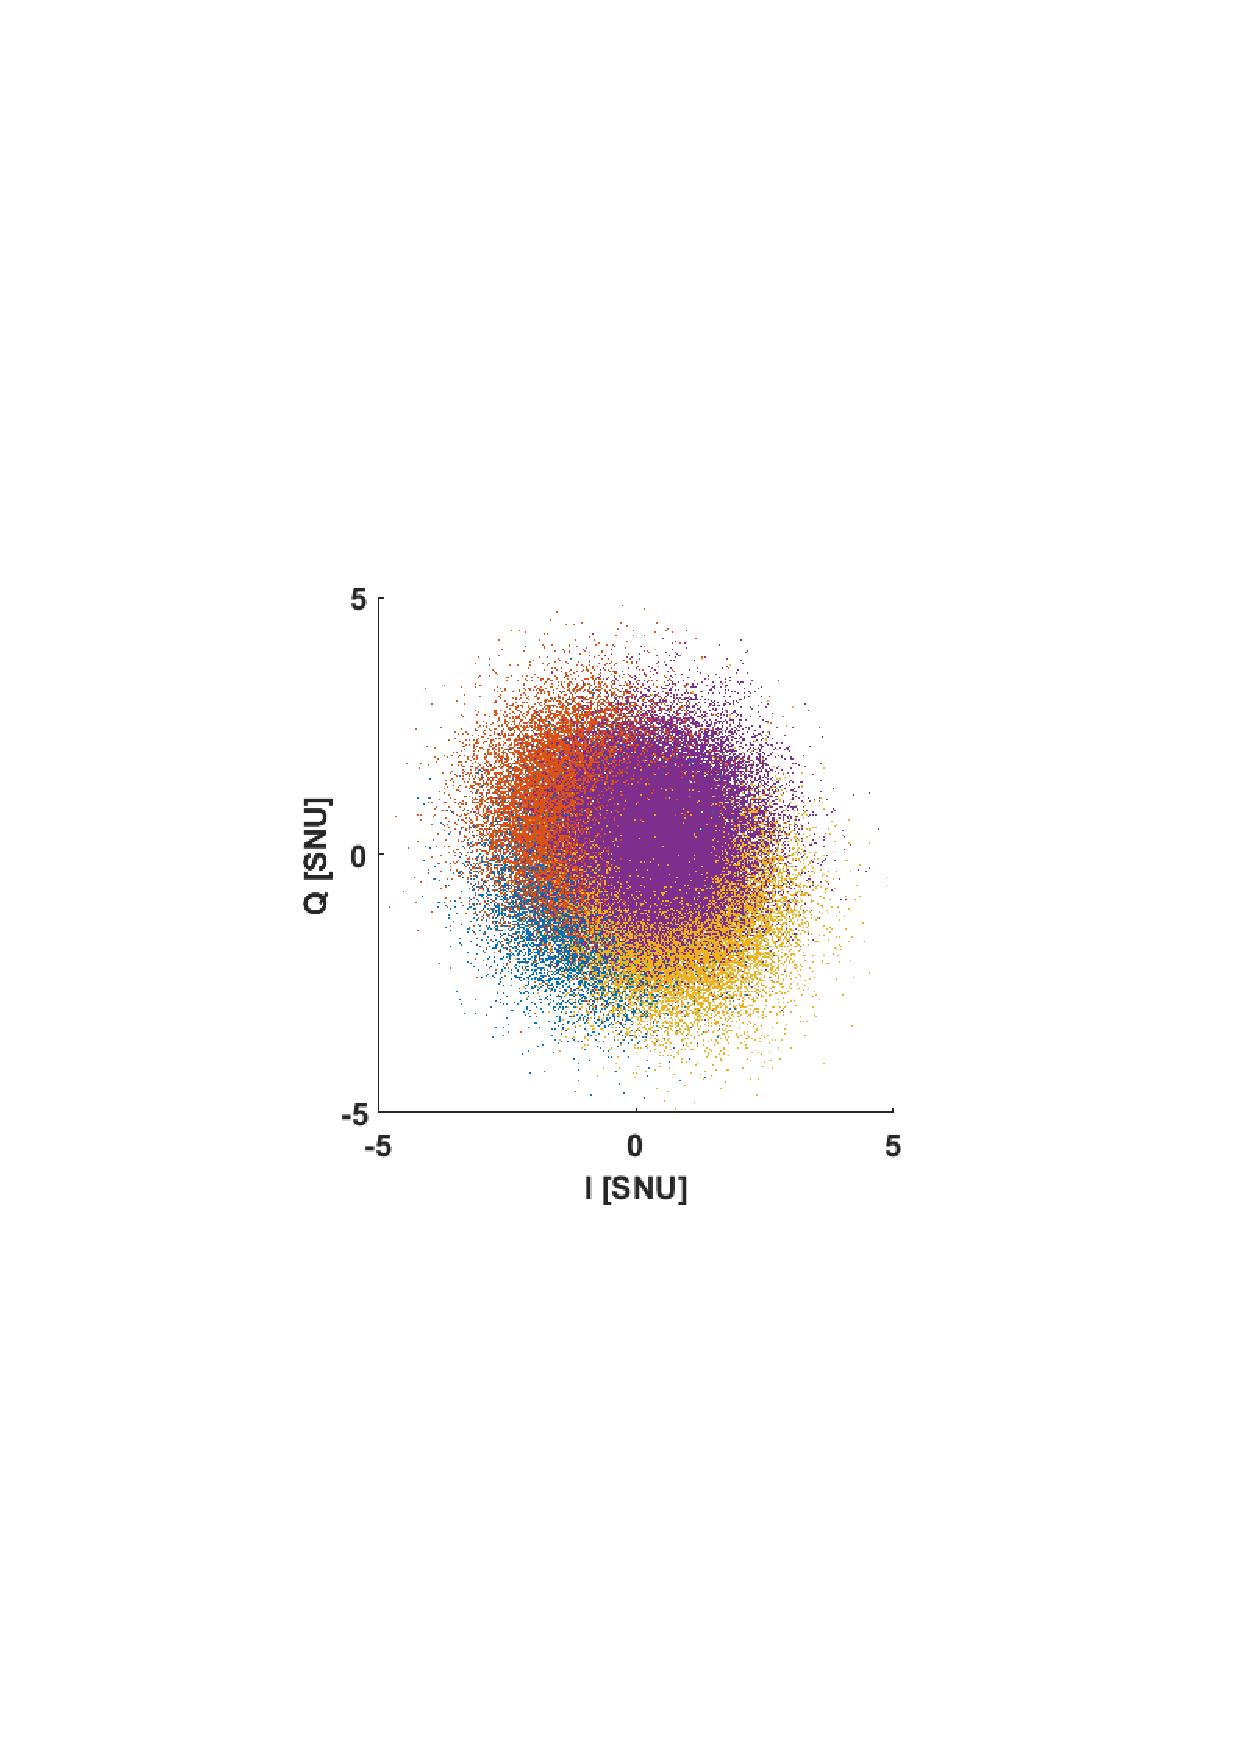
\includegraphics[width=\linewidth, trim={3cm 9cm 3cm 9cm}, clip=true]{singleQBTBSNU.pdf}
 Single laser, BTB recovered constellation\\
\end{center}
\end{minipage}% This must go next to `\end{minipage}`
\begin{minipage}{.5\textwidth}
\begin{tabular}{l|c|c}
$\epsilon$[SNU] &   \multicolumn{2}{c}{0.074}  \\ \hline
 & \textbf{Theo} & \textbf{Exp} \\ \hline
$T$ & Efficiency & 0.9519 \\ \hline
$K\left[\frac{\text{bits}}{\text{symb}}\right]$ & 0.0288 & 0.0213
\end{tabular}
\end{minipage}

%--------------------------------------------------------------------------------------------------
%------------ SLIDE-------
\mysection{Experimental results - System performance}\large
\vspace{0cm}

\noindent
The system's performance was evaluated for 4 different setups, utilizing a single/double laser setup coupled with either a direct connection or a 10~km transmission channel. The secret key rate was estimated through the finite size analysis presented before.

\begin{minipage}{.5\textwidth}
\begin{center}
 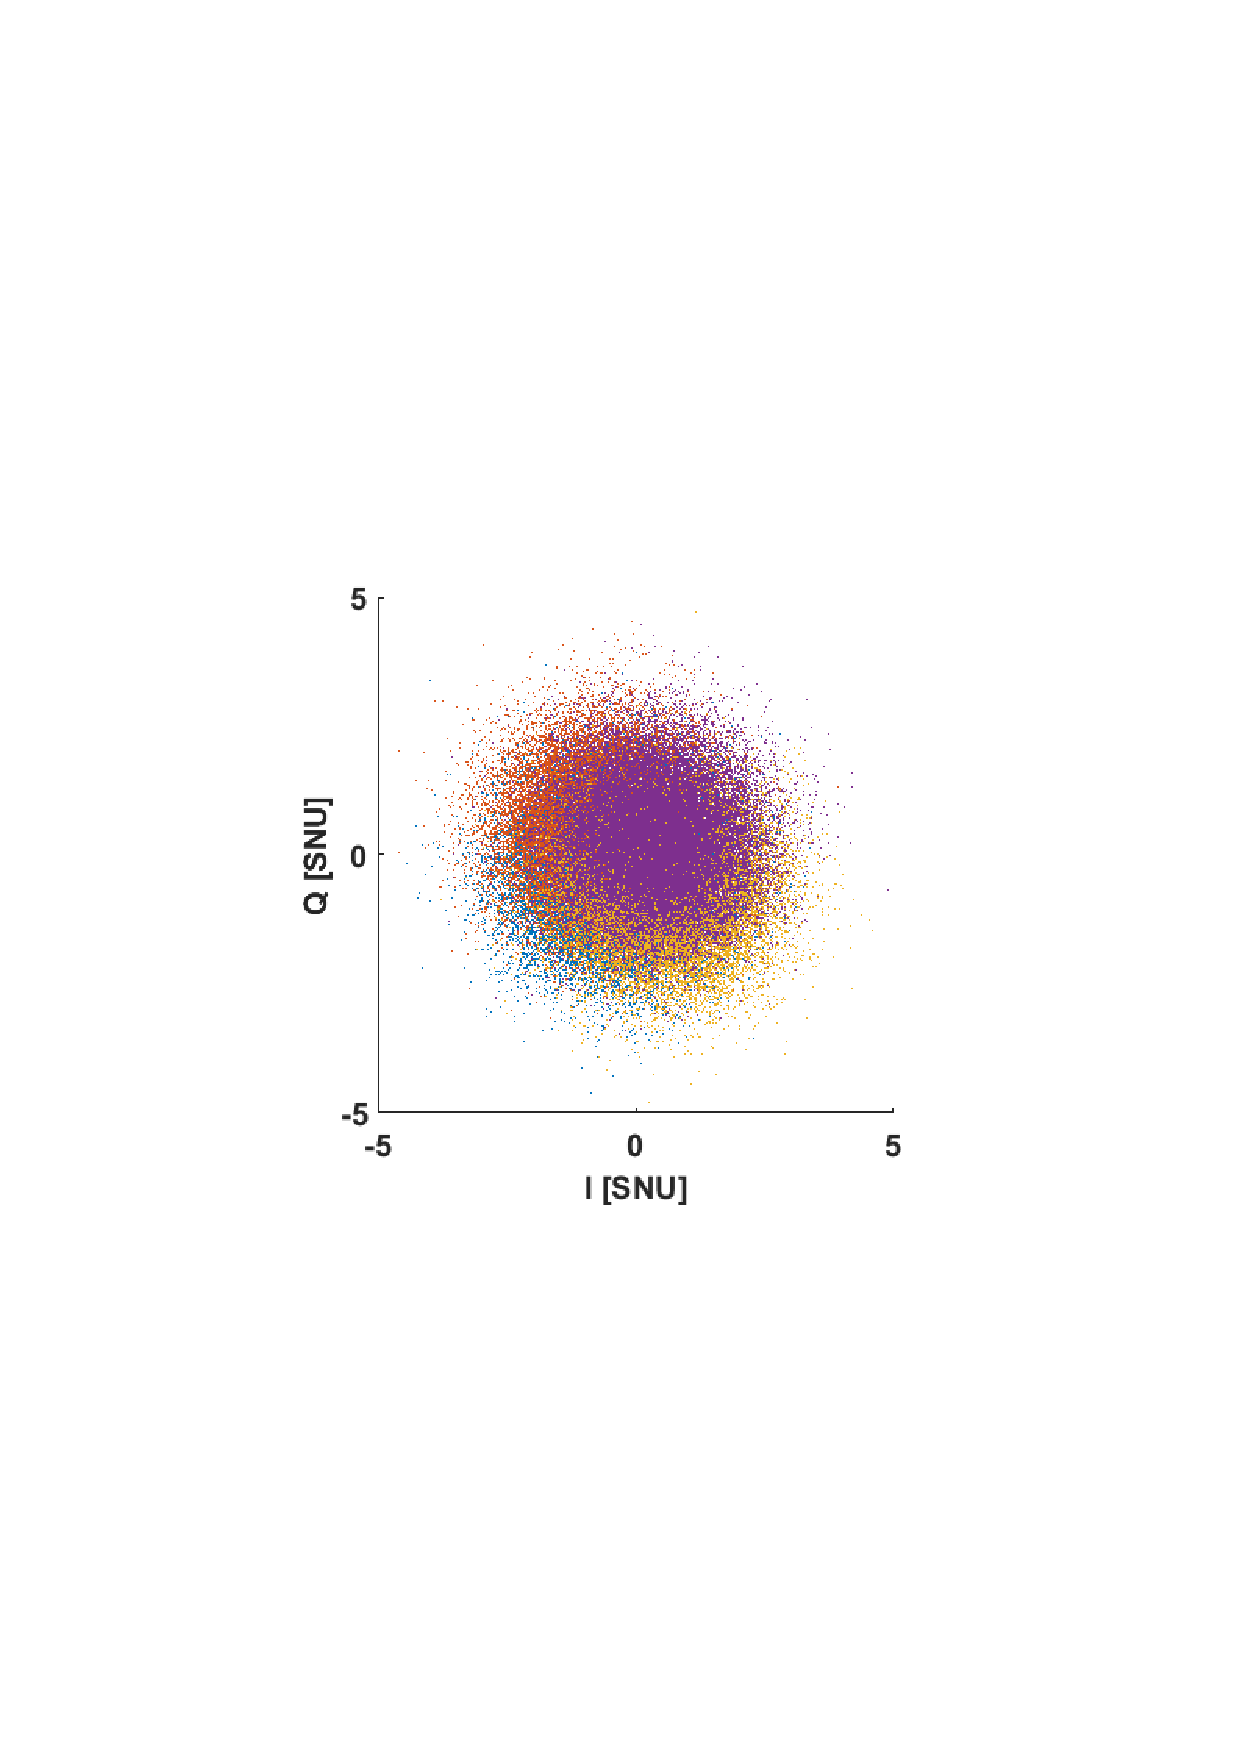
\includegraphics[width=\linewidth, trim={3cm 9cm 3cm 9cm}, clip=true]{singleQ10kmSNU.pdf}
 Single laser, 10~km recovered constellation\\
\end{center}
\end{minipage}% This must go next to `\end{minipage}`
\begin{minipage}{.5\textwidth}
\begin{tabular}{l|c|c}
$\epsilon$[SNU] &   \multicolumn{2}{c}{0.0156}  \\ \hline
 & \textbf{Theo} & \textbf{Exp} \\ \hline
$T$ & 0.4547 & 0.4317 \\ \hline
$K\left[\frac{\text{bits}}{\text{symb}}\right]$ & 0.0132 & 0.0094
\end{tabular}
\end{minipage}


%--------------------------------------------------------------------------------------------------
%------------ SLIDE-------
\mysection{Experimental results - System performance}\large
\vspace{0cm}

\noindent
The system's performance was evaluated for 4 different setups, utilizing a single/double laser setup coupled with either a direct connection or a 10~km transmission channel. The secret key rate was estimated through the finite size analysis presented before.

\begin{minipage}{.5\textwidth}
\begin{center}
 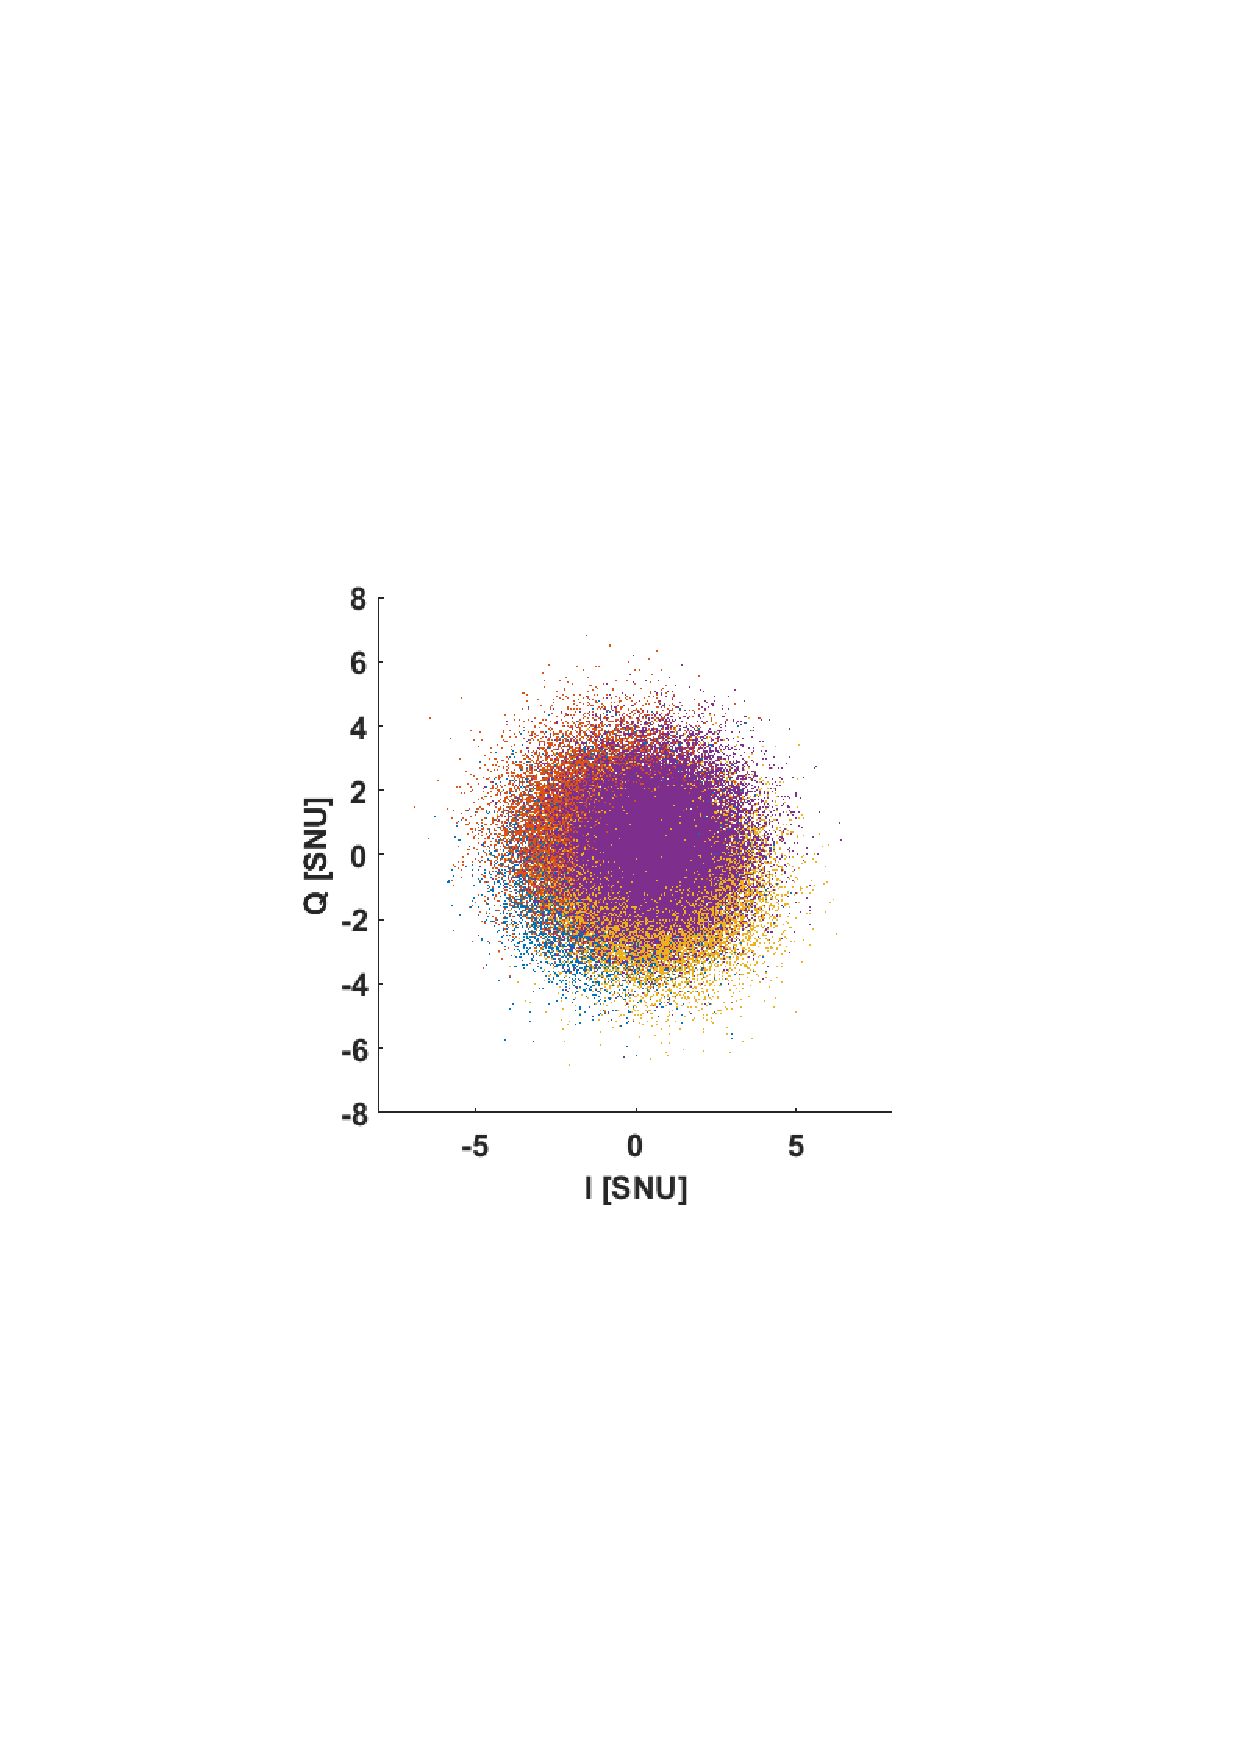
\includegraphics[width=\linewidth, trim={3cm 9cm 3cm 9cm}, clip=true]{doubleQBTBSNU.pdf}
 Double laser, BTB recovered constellation\\
\end{center}
\end{minipage}% This must go next to `\end{minipage}`
\begin{minipage}{.5\textwidth}
\begin{tabular}{l|c|c}
$\epsilon$[SNU] &   \multicolumn{2}{c}{2.9915}  \\ \hline
 & \textbf{Theo} & \textbf{Exp} \\ \hline
$T$ & $\sim$0.95 & 0.9557 \\ \hline
$K\left[\frac{\text{bits}}{\text{symb}}\right]$& Negative & -0.8011
\end{tabular}
\end{minipage}


%--------------------------------------------------------------------------------------------------
%------------ SLIDE-------
\mysection{Experimental results - System performance}\large
\vspace{0cm}

\noindent
The system's performance was evaluated for 4 different setups, utilizing a single/double laser setup coupled with either a direct connection or a 10~km transmission channel. The secret key rate was estimated through the finite size analysis presented before.

\begin{minipage}{.5\textwidth}
\begin{center}
 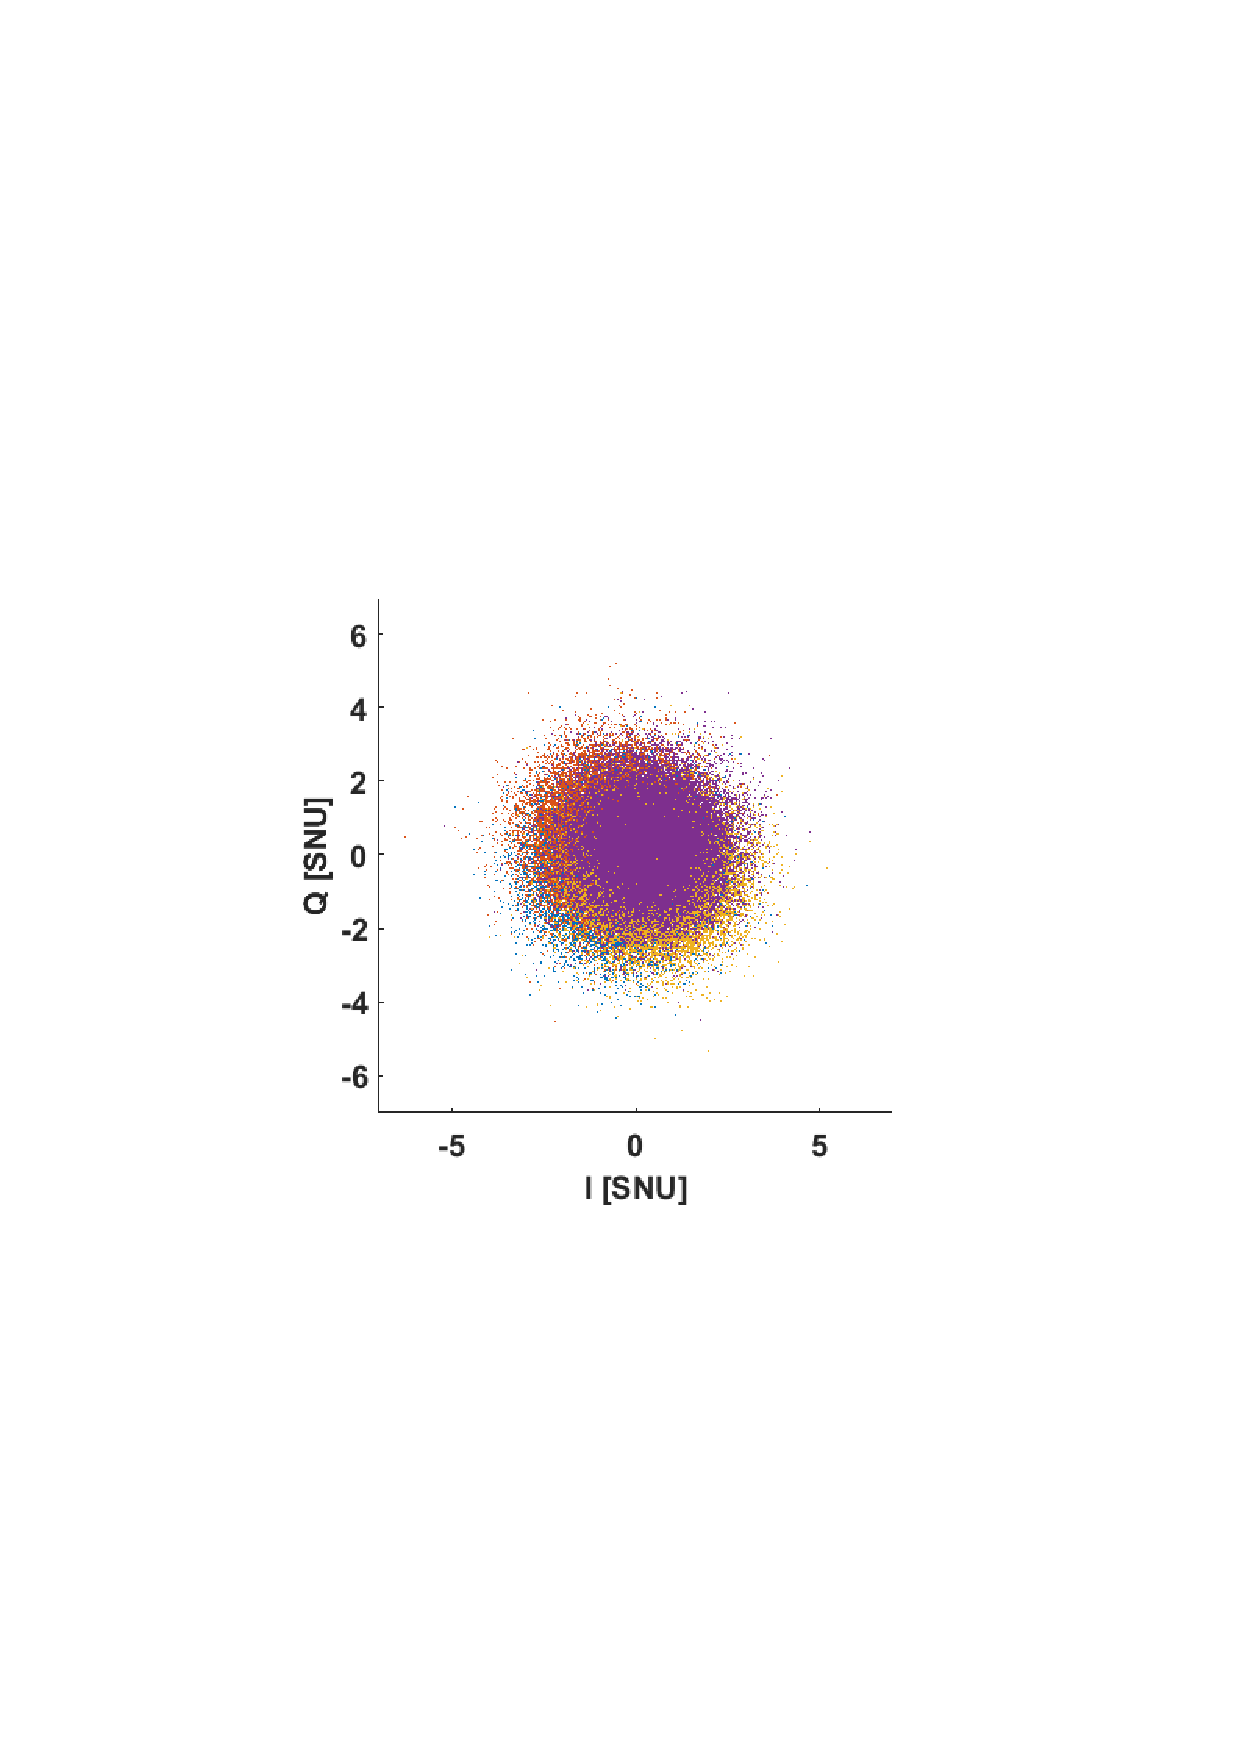
\includegraphics[width=\linewidth, trim={3cm 9cm 3cm 9cm}, clip=true]{doubleQ10kmSNU.pdf}
 double laser, 10~km recovered constellation\\
\end{center}
\end{minipage}% This must go next to `\end{minipage}`
\begin{minipage}{.5\textwidth}
\begin{tabular}{l|c|c}
$\epsilon$[SNU] &   \multicolumn{2}{c}{2.8196}  \\ \hline
 & \textbf{Theo} & \textbf{Exp} \\ \hline
$T$ & 0.4547 & 0.4282 \\ \hline
$K\left[\frac{\text{bits}}{\text{symb}}\right]$ & Negative & -0.4769
\end{tabular}
\end{minipage}


\end{document}
